%\documentclass[acmjacm,acmnow]{acmtrans2m}
%\documentclass[conference,final]{IEEEtran}
%\documentclass[10pt,letterpaper]{article}
\documentclass[preprint,12pt]{article}

\usepackage{graphicx}
\usepackage{url}
\usepackage{color}
\usepackage{pdfsync}

% \acmVolume{}
% \acmNumber{}
% \acmYear{}
% \acmMonth{}


%\usepackage{sectsty}
%\usepackage{setspace}

% \usepackage{ifpdf}
% \usepackage{wrapfig}
% %\usepackage[cm]{fullpage}
% \usepackage{textcomp}
% \usepackage{srcltx}
% \usepackage{fancyhdr}
% \usepackage{setspace}
\usepackage{lscape}
% \usepackage{longtable}
% \usepackage{paralist}

%\usepackage{hyperref}
%\usepackage{pdfsync}

% \usepackage{ams}

% \ifpdf    %   \usepackage[pdftex,
%               colorlinks=true,
%               linkcolor=red,
%               citecolor=red,
%               filecolor=red,
%               ]{hyperref}
% \else
%   \usepackage[hypertex]{hyperref}
% \fi

% Space saving
%\usepackage[small,compact]{titlesec}
%\usepackage[small,it]{caption}

% \renewcommand\floatpagefraction{.9}
% \renewcommand\topfraction{.9}
% \renewcommand\bottomfraction{.9}
%\renewcommand\textfrare{.1}

\setcounter{totalnumber}{50}
\setcounter{topnumber}{50}
\setcounter{bottomnumber}{50}

%\textwidth = 6in
%\textheight = 8.5 in
%\oddsidemargin = 0.0 in
%\evensidemargin = 0.0 in

% \topmargin = 0.0 in
% \headheight = 0.0 in
% \headsep = 0.0 in
%\parskip = 0.0in
%\parindent = 0.5cm
\parskip = 0.04in
% \parindent = 0.0cm
% \textfloatsep = 0.1in

% \usepackage[draft,pdftex,colorlinks=true, linkcolor=blue,citecolor=blue,
%        urlcolor=blue]{hyperref}

% \ifpdf
% \pdfinfo{ /Author (Shantenu Jha et al.)  /Title (Programming Abstractions for Large-Scale Distributed Applications) }
% \fi

\newcommand{\projectnamefull}{\textit{Programming Abstractions for
    Large-Scale Distributed Applications} }

\newcommand{\upup}{\vspace*{-0.5em}}
\newcommand{\up}{\vspace*{-0.25em}}
\newcommand{\I}[1]{\textit{#1}}
\newcommand{\B}[1]{\textbf{#1}}
\newcommand{\T}[1]{\texttt{#1}}
\newcommand{\BI}[1]{\B{\I{#1}}}

% \ifpdf
%   \DeclareGraphicsExtensions{.pdf, .png, .jpg}
% \else
%   \DeclareGraphicsExtensions{.ps, .eps}
% \fi

\long\def\comment#1{{\bf \textcolor{magenta}{\bf #1}}}
\long\def\ccomment#1{{\bf \textcolor{blue}{\bf #1}}}
\newcommand{\C}{\comment}
\newcommand{\CC}{\ccomment}

\newcommand{\yes}{$\bullet$}

\long\def\finalcomment#1{{\bf \textcolor{red}{\bf #1}}}
\newcommand{\CF}{\finalcomment}

\newif\ifdraft
\drafttrue
\ifdraft
 \newcommand{\katznote}[1]{ {\textcolor{magenta}    { ***Dan:      #1 }}}
 \newcommand{\rananote}[1]{ {\textcolor{blue}    { ***Omer:     #1 }}}
 \newcommand{\note}[1]{ {\textcolor{red}    { #1 }}}
\newcommand{\manishnote}[1]{{\textcolor{green}   { ***Manish:   #1 }}}
\newcommand{\jhanote}[1]{  {\textcolor{blue}     { ***Shantenu: #1 }}}
 \newcommand{\jonnote}[1]{  {\textcolor{red}      { ***Jon: #1 }}}
\else
 \newcommand{\katznote}[1]{}
 \newcommand{\rananote}[1]{}
 \newcommand{\note}[1]{}
 \newcommand{\manishnote}[1]{}
 \newcommand{\jhanote}[1]{}
 \newcommand{\jonnote}[1]{}
\fi

\title{3DPAS: Distributed Dynamic Data-intensive Programming
  Abstractions and Systems}

%\author{J.D. Blower$^{10}$, Neil Chue-Hong$^{}$, Simon Dobson$^{}$,
%  Shantenu Jha$^{1,2,3}$, Daniel S. Katz$^{4,1,5}$, Omer Rana$^{8}$}

\footnotesize{\author{Editors: J.D. Blower, Neil Chue-Hong, Simon Dobson, \\[-0.1em]
  Shantenu Jha, Daniel S. Katz, Omer Rana}}

%Manish Parashar$^{6,7}$,
%   Jon Weissman$^{9}$,

%   \small $^1$Center for Computation \& Technology,
%   Louisiana State University\\[-0.1em]
%   \small $^2$Department of Computer Science,
%   Louisiana State University\\[-0.1em]
%   \small $^3$e-Science Institute,   University of Edinburgh\\[-0.1em]
%   \small $^4$Computation Institute,   University of Chicago\\[-0.1em]
%  \small $^5$Department of Electrical and Computer Engineering,
%   Louisiana State University\\[-0.1em]
%   \small $^6$NSF Center for Autonomic Computing, Rutgers University\\[-0.1em]
%   \small $^7$Department of  Electrical and Computer Engineering, Rutgers University\\[-0.1em]
%   \small $^8$Department of Computer Science,
%   Cardiff University\\[-0.1em]
%   \small $^9$Department of Computer Science,
%   University of Minnesota\\[-0.3em]
%   \small $^10$Reading e-Science Centre, University of Reading, UK
%}
\begin{document}
\maketitle

\begin{abstract}
\footnotesize{Many problems at the forefront of science, engineering, medicine,
  and the social sciences, are increasingly complex and
  interdisciplinary due to the plethora of data sources and
  computational methods available today.  A common feature across many
  of these problem domains is the amount and diversity of data and
  computation that must be integrated to yield insights. Such data is
  increasingly large-scale and distributed;
  the data-sets, their location and scheduling decision
  are time-dependent. % Applications need access
  % to these disparate data-sets and to the methods that operate on
  % them.  Data-intensive applications need first-class support for
  % distributed heterogeneous platform execution.
  The 3DPAS Research theme (funded by the eSI, Edinburgh and US NSF),
  aims to investigate applications that have these characteristics, in
  other words it operates at the triple point of {\it dynamic} and
  {\it distributed} and {\it data-intensive}, (3D) attributes.  This
  evolving document represents work in progress of the 3DPAS Research
  Theme.}
\end{abstract}

%\input{notes}

\begin{figure*}[htbp]
  \begin{center}
    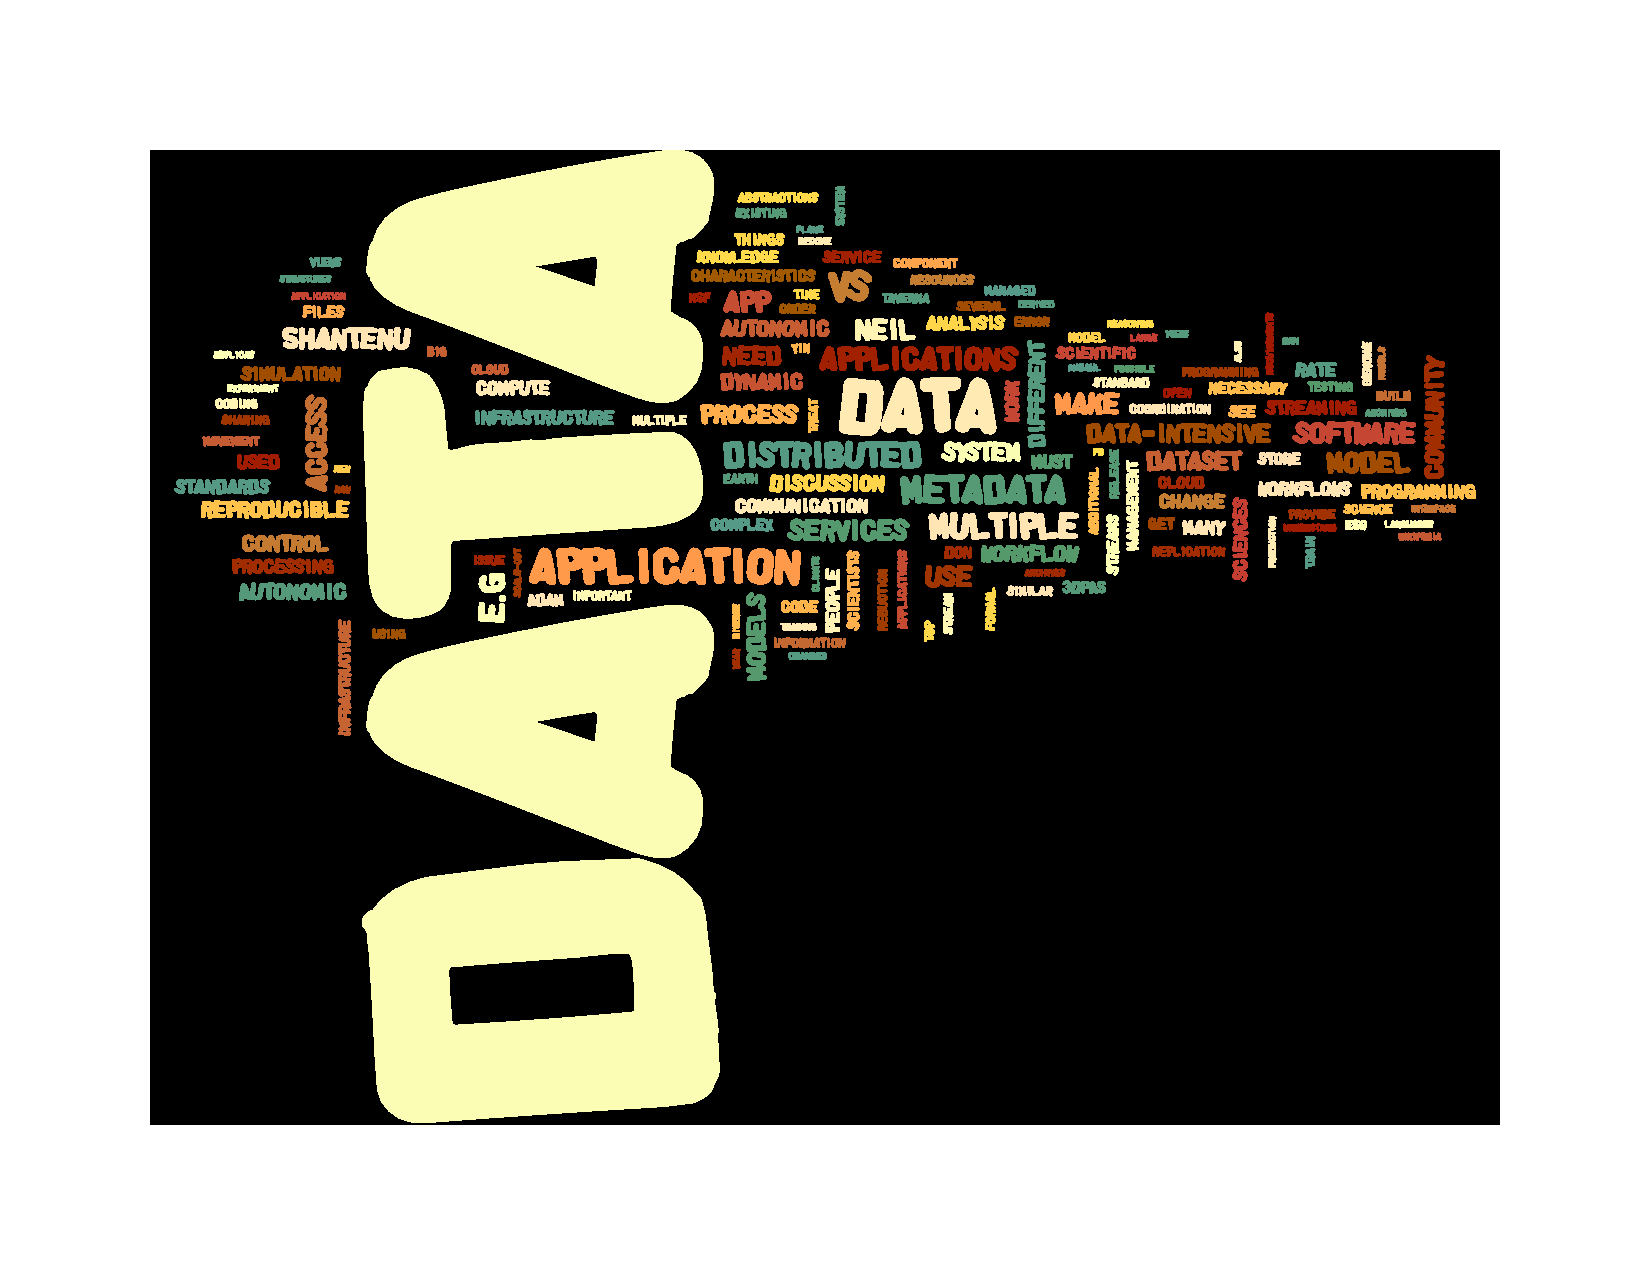
\includegraphics[scale=0.33]{figures/3dpas-wordle.pdf}
    \caption{Wordle of 3DPAS document}
    \label{Fig:wordle}
  \end{center}
\end{figure*}


\section{Introduction: Context, Scope and Outline}

The NERC\footnote{UK Natural Environment Research Council} Virtual
Observatory\footnote{http://www.nerc.ac.uk/research/programmes/virtualobservatory/}
is a new initiative to create a pilot cloud-based environment in which
different practitioners will discover, visualize and process data
relating to the UK's system of rivers and soils.  It will provide
access to many different kinds of distributed hydrological data,
including sensor data and numerical models, many of which produce
rapidly-changing, dynamic information.  There are many scientific
challenges to be faced, notably including the coupling of the models
and observations; this includes the possibility that sensors can be
dynamically tasked in response to model forecasts, or that models may
adapt dynamically to new information from sensors.  Principles of the
Web and ``linked data'' may help to solve some of the challenges in
informatics, but many technical challenges will remain regarding the
handling of dynamic data, including keeping careful records of its
provenance in order to record the steps taken in making a decision.


\section{Understanding Distributed Dynamic Data}

Why bother about distributed, dynamic and data-intensive applications?

\subsection{Importance of Distributed}

\subsection{Importance of Dynamic and Examples}

\subsubsection{Types of Dynamic Data}

\begin{enumerate}
\item Streaming data -- data comes and goes
  \url{http://traffic.berkeley.edu/} and \url{http://lagrange.ce.berkeley.edu/fsn/}
\item Data set that is being operating upon is changing
\item Data has to be transformed
\item Placement decisions time-dependent
\end{enumerate}

\jhanote{We should highlight which of the above dynamic case are to be
  found in applications}

\katznote{Question: is there anything unique about scientific work on streaming data?  Or is all work on streaming data basically them same, whether it's in science or finance, for example?}

\subsubsection{Dynamic Data in a Web Environment}\label{sec:dynamicdataweb}
\emph{Just some placeholder notes from Jon.  Could belong elsewhere.}

Web Services are commonly used to distribute data through HTTP.  A key characteristic of dynamic data, of course, is that it changes with time.  It is of great importance for the user to be confident that she is accessing the correct version of the data; this will often be the most up-to-date data, or may be a specific historical version.  In a Web environment, servers and proxy servers (which are sometimes beyond the control of the data provider or the data user) may retain caches of data in a strategy to reduce server load and network traffic.  For this reason, the HTTP protocol provides mechanisms for defining expiry times for data resources, specifying when a resource ought to be cleared from the cache.

In the environmental and geospatial communities the Open Geospatial Consortium specifications are being widely adopted alongside existing protocols such as OPeNDAP.  Unfortunately these protocols, although built atop HTTP, do not make it easy for this versioning to be implemented correctly.  The OPeNDAP protocol does not have the concept of a dataset version, meaning that clients have no reliable or efficient means to detect that a dataset has changed.  The OGC protocols in general [TODO: look into this], \emph{do} provide versioning at the level of the service endpoint, but provide no information on when a resource should be considered expired.  Clients are therefore forced to poll the server to check for updates.

Therefore we see that in a ``pull'' environment such as the Web, it is necessary for servers to advertise not only the version of a resource, but also the expiry time in order to handle dynamic data correctly.  The frequency of updates is also useful information for service consumers.  Expiry times can be specified using the mechanisms of HTTP (although this capability is often not used in practice), but resource versioning and update frequency must be handled at a higher level.

[All this must be fairly well-known and almost certainly covered in the literature, with the possible exception of the material on OPeNDAP and OGC.  Any references we could cite?]

\subsection{Other points to cover}

\begin{itemize}
\item Lay out several scenarios first, and then formulate/define Dynamic Data
\item Dynamic: transformed by the workflow scenario (state is captured by immutable objects)
\item How does this differ from Scientific Databases
\item How does it relate to Scientific Data Management and Scientific data flow
\item Carve out the specifics of this theme -- and how it relates to such existing approaches (a diagram would be nice)
\item Underlying data model (operations) are highly domain specific -- make clear what can be domain specific and domain independent
\item Relationship to ``legacy''
\item Dynamic data can arise at different levels (application vs. middleware (infrastructure)). Identify which is the primary consideration here, and what is different.
\item Reference to EU 2030 Objectives (part of the Project Europe 2030
  Report) -- underpins ``Data Intensive Research'' from an EU
  perspective (strategy) + relate this to NSF ``CIF21'' vision
\end{itemize}

How does Dynamic Data relate to Distributed \& ``Big'' Data? Relate to
DPA and Malcolm et al.'s theme (Data Lifecycle, Complexity, etc)


\section{Application Scenarios} {\bf Dan, Shantenu (co-leads), All}

Application Scenario Characteristics for Dynamic Data (Various)

Identify: (1) what is the case scenario within the application; (2) what data is dynamic; (3)  how the data is being used in the context of each of these scenarios.

Currently trying to do this by asking the following questions:
\begin{enumerate}
\item What is the purpose of the application?
\item How is the application used to do this?
\item What infrastructure is used? (including compute, data, network, instruments, etc.)
\item What dynamic data is used in the application?
\begin{enumerate}
\item What are the types of data,
\item What is the size of the data set(s)?
\end{enumerate}
\item How does the application get the data?
\item What are the time (or quality) constraints on the application?
\end{enumerate}


\subsection{Silvia's Biosciences app: NGS, medical imaging (Silvia)\label{bioSilvia}}

\begin{itemize}
\item Infrastructure monitoring for the execution of workflows to
  manage failure
\item the application is sequence alignment (split data (this is where there is dynamic decision making) to execute the alignment in parallel)
\item DTI Imaging: two cases are interesting: DTI atlas (split, run, merge, split, merge - reduction from 10000 tasks to 1 output); PCA for classification of patients/control
\end{itemize}

\subsubsection{Silvia's contribution}

NGS sequence alignment on the AMC e-bioscience infrastructure

1. What is the purpose of the application?

The application performs analysis of DNA sequencing data for various
goals in life science research, e.g., Mutation screening, Virus
discovery, Genome-wide Associations (GWA), Linkage analysis,
Comparison of bacterial genomes, microRNA expression and Exome
sequencing. The data analysis is composed of various methods that are
implemented by a bioinformatician, whereas the data is typically owned
by the life scientist.

2. How is the application used to do this?

Note: Here we focus on data analysis from the perspective of the
bioinformatician, excluding steps related to data acquisition
(transformation of raw images into sequences of amino acids) and
posterior biostatistics and epidemiological analysis.

The data analysis is implemented as a pipeline of generic and
customized components, mostly third-party public software tools. The
pipeline may differ for each specific study, depending on the data
acquisition and the research question. Typically it includes data
preparation (file conversion, reformatting and filtering); alignment
(comparison) with some reference database as the human genome;
post-processing (output conversion, reformatting, statistical
analysis) and visualization. Sequence alignment is the most
computing-intensive step, which became prohibitive for sequential
execution in next generation sequence experiments. All data is stored
in files that are often completely read in memory for fast
processing. Compressed formats are usually adopted. Although the files
are large, the data can be easily decomposed because the processing is
done on each sequence (`string') at a time.


3. What infrastructure is used? (including compute, data, network,
instruments, etc.)

\begin{figure*}[htbp]
  \begin{center}
    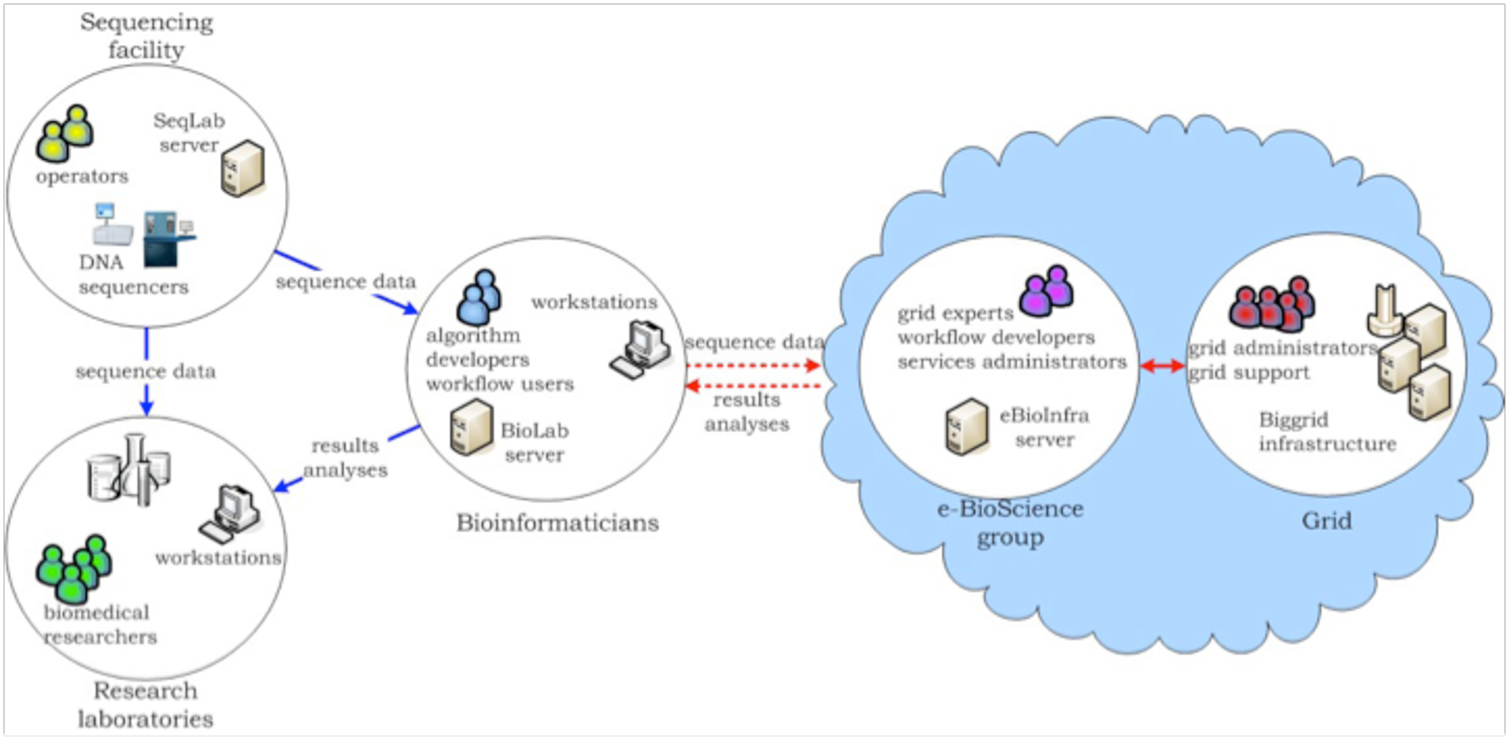
\includegraphics[width=\textwidth]{figures/silvia.pdf}
    \caption{Figure from Silvia}
    \label{Fig:silvia}
  \end{center}
\end{figure*}


see Figure~\ref{Fig:silvia}.

Data:

Data acquisition: Roche, Solid and Illumina next generation sequencers

Local storage: dedicated server at the AMC network (ftp)

Grid storage: Storage Elements of the Dutch e-Science Grid
(www.biggrid.nl)

Data transport:

From sequencer to server: AMC network (XXX) or off-line media

Between data server and grid storage: public network (XXX); lightpath
(near future)

Between grid storage and worker nodes: public (XXX) or site (XXX)
network

Computing:

Local Computing: clusters and servers at the AMC and workstations
(laptops, desktops) anywhere Grid Computing: Dutch Grid
(www.biggrid.nl), part of EGI

Originally all steps were performed in some local server or on the
user's workstation. The visualization is still performed in the user's
(windows) workstation, but all the other steps are currently performed
on the Dutch grid infrastructure. The pipeline is described as a grid
workflow using the GWENDIA language
(\url{http://dx.doi.org/10.1145/1645164.1645171}) and enacted on the
Dutch Grid using the MOTEUR2 workflow engine
(\url{http://modalis.polytech.unice.fr/softwares/moteur/start}).

PS: although only the alignment step is computation-intensive, it is
more practical to perform all the others on the grid to minimize data
transport to/from the user's workstation, which is normally on low
speed networks. That is, the computation is statically and manually
taken to the data in this case. This can lead to sub-optimal resource
usage.

4. What dynamic data is used in the application?

Note: data is not really `dynamic' in this case -- the sequences are
acquired once and analyzed many times. However the execution of this
application on a distributed infrastracuture has dynamic aspects when
optimized resource usage is considered:

\begin{itemize}
\item Split/merge the data according to available resources
\item Compute resource selection based on data location, processing profile and/or network capacity
\item Resource selection based on security constraints (access control, trust)
\item Collection and processing of monitoring information to steer grid enactment.
\end{itemize}

(a) What are the types of data,

DNA sequences (strings) stored in open formats (FASTA, SFF, SAM, BAM)
Bundles of results from alignment tools (custom format, binary?)

(b) What is the size of the data set(s)?

one example for BWA alignment tool (short sequences) follows:

input data: Sequencing Data in the csFasta format, normally 25-35~GB;
Quality files in the .qual format, normally 50-80~GB;
Reference DB in the Fasta BS format: 3.2~GB (human genome) 140~MB (one chromosome)

Intermediate files:
Reference BWA index, normally 4.5GB (human genome) 240~MB (one chromosome);
Sequencing Data in the FastQ format (fastq.gz), normally 20-30~GB

Output:
Results in .sai format (direct output of BWA), normally 2-3~GB;
Results in .sam format, normally 55-75~GB;
Results in .bam format, normally 20-30~GB

5. How does the application get the data?

From a local file. The legacy code is wrapped to stage the inputs and outputs in/out the worker node.

All data is stored in files that are often completely read in memory
for fast processing. Compressed formats are usually adopted. Although
the files are large, the data can be easily decomposed because the
processing is done on each sequence (`string') at a time

6. What are the time (or quality) constraints on the application?

In research there are no strict constraints on the time to complete
the analysis.  In patient care, time could determine life, death or
money, but we have no concrete case yet.

Quality in this case refers to the accuracy of the results
obtained. This is essential for research and patient care.

\subsection{WLCG (focus on ATLAS) (Steve Fisher) \label{WLCGSteve}}
\begin{itemize}
\item Most of the dynamism is in infrastructure, not in the application (e.g. use of PilotJob)
\item Application dynamism: location of file (e.g. if file turns out to be not local, look up in registry-- but not do this again)
\item No specific QoS issue concerned with data transfer times
\end{itemize}

\subsubsection{Answers from Steve}

3DPAS - Particle Physics - the example of Atlas physics channel
selection.

   1.  What is the purpose of the application?

A physics group is interested in a specific physics channel
(underlying physical process) as recorded by the Atlas experiment at
the LHC (Large Hadron Collider) at CERN in Geneva. The set of
available data grows steadily over time as more data are collected and
reconstructed.

   2.  How is the application used to do this?

 Both physics groups and individuals run jobs as they see fit, either
reading the reconstructed data or reading intermediate datasets
created by themselves or their colleagues. If, in the future,
resources should prove inadequate then adjustments to working
practices to coordinate processing may be made to increase physics
output.

   3.  What infrastructure is used? (including compute, data, network,
instruments, etc.)

The WLCG (Worldwide LHC (Large Hadron Collider) Computing Grid) is
used with a mixture of gLite software, experiment specific software
and physics group specific software. WLCG has 250,000 cores
distributed over 140 sites and with 100PB of disk. CERN is connected
to the eleven `Tier 1' national sites by a dedicated optical
network. This may be extended in the future.

   4.  What dynamic data is used in the application?

The data being processed can be considered as dynamic as it grows
steadily as new raw data are collected and the basic reconstruction
program is run to produce information about specific particles
involved in a collision. This reconstruction is rerun periodically
(two or three times per year is expected) as calibrations of the
detector are improved. Reconstruction algorithms are also improved as
are the physics groups' selection codes. One output of the
reconstruction is `tag' data - summary information written to a
database to facilitate event selection. This is not yet used very
much. Calibration data are held on an RDBMS with Frontier/Squid front
ends.

         a.  What are the types of data,

          The bulk of the data is individual event data at different
stages of refinement. This is held in a in-house representation of C++
serialized objects. Though this format is not standard it is used by
all LHC experiments.

         b.  What is the size of the data set(s)?

          Roughly 20~TB of data are collected every day. Multiple
generations of processed data are kept. Many data files are replicated
on multiple sites; this is done both by copying it to where it is
likely to be useful and partly dynamically as the need arises.

   5.  How does the application get the data?

A copy of the file is made to the SE (Storage Element) at the site
where the job will run. From there it is either copied to a local disk
or read from the SE.

   6.  What are the time (or quality) constraints on the application?

If some data are missed during processing the only effect is a
reduction of statistical precision in the final analysis. Accurate
book keeping is important to know which data have been processed. If
the selection code has been improved then naturally the physics groups
would like to see the results as soon as possible.



\subsection{Astrophysics -- Virtual Observatory
(Bob) \label{astroBob}}
\begin{itemize}
\item Analysis of data to generate event streams $\rightarrow$ lead to
the positioning of telescopes
\end{itemize}

\subsubsection{Answers from Bob}

I assume that the ``application'' in question is the sum of the two
activities, despite the fact that they are different in many respects,
and I try and distinguish between them where appropriate.

1. What is the purpose of the application?

An increasingly important feature of astronomical research is the
existence of systematic sky surveys covering the whole sky (or large
fractions thereof) in many different wavebands. The principal outcome
from these surveys are astronomical source catalogues, which contain
values for attributes characterizing all the celestial sources
detected in the sky survey dataset.  These are now typically
implemented in relational databases, with SQL interfaces implemented
through web pages, and the principal goal of the Virtual Observatory
(VO) is to standardize access to these, and other astronomical data
resources, so that astronomers can readily perform multi-wavelength
analyses, combining all the extant data on particular sources.

      2. How is the application used to do this?

The VO includes a registry that contains metadata describing all the
data resources published using VO data access standards, enabling the
discovery of datasets relevant to a particular analysis. Web service
implementations of data access protocols enable users to access data
in these repositories programmatically, and distributed scratch space
is provided for the storage of intermediate result sets, so the user
does not need to route large data flows through his/her own
workstation. In the future, more and more data analysis software will
be made available through web services compliant with VO standards,
enabling more of the data integration and analysis process to be
combined in workflow.

      3. What infrastructure is used? (including compute, data,
network, instruments, etc.)

The data resources published to the VO exist in a number of data
centers distributed internationally. Major datasets---e.g. those from
large sky surveys---are typically implemented in relational databases
running on high-spec servers or clusters thereof. The compute
requirements of the VO are currently modest, but are likely to
increase over time. Astronomers typically use normal academic
networks, but more specialized networking is required in some cases:
e.g., sky survey data is moved from Cambridge to Edinburgh using the
UKLight project's dedicated optical network, and radio interferometers
require high-bandwidth fibre connections from each antenna to the
correlator.

      4. What dynamic data is used in the application?  (a) What are
the types of data, (b) What is the size of the data set(s)?

The VO currently includes little dynamic data. The one exception is
VOEvent messages, which are notifications of transient events which
can be used to trigger follow-up observations on other
telescopes. These are small XML messages containing basic information
about the position of a transient source and a small amount of other
metadata which the operators of a given telescope can use to define
triggers for follow-up observations of interest to them or their
community.

 5. How does the application get the data?

Assuming this refers solely to the dynamic data, then a number of
telescopes undertaking real-time detection of transient events emit
VOEvent messages through feeds to which other parties can subscribe.

6. What are the time (or quality) constraints on the application?

The time constraints differ for different types of transient source,
but in some cases notification must be made within a few minutes if it
is to be useful; the overheads associated with setting up a follow-up
observation mean that much shorter time scales are practically
irrelevant, although they are still scientifically interesting. The
quality constraints centre on providing a telescope with good enough
information about a potential transient source that it can make a
reliable decision about whether to interrupt its existing observing
program to follow-up the event. In most cases, the candidate transient
will be some sort of noise event, so fairly sophisticated filtering is
required to bring the false positive rate down to something
acceptable, given the cost of observing time on cutting edge
telescopes.


\subsection{Sensor Network App (Simon) \label{sensorSimon}}

\begin{itemize}
\item Environmental (Marine) -- sensing within a hostile environment,
data quality + availability of communication infrastructure (Simon)
\item Patient monitoring -- data quality, type of data to transmit
(Omer)
\end{itemize}

\subsubsection{Answers from Simon}

1. What is the purpose of the application?

Marine sensing covers a range of different applications, including
environmental monitoring, remote exploration, marine life surveys and
habitat assessment. In each case, the main challenges are collecting
data reliably in what is an extremely challenging technical
environment---far more so than in air---and (in the case of biological
surveillance), without interfering with the natural behaviors the
animals exhibit.

2. How is the application used to do this?

At present most applications are quite small-scale. A canonical
example is the monitoring of seal and other sea mammal populations by
the Scottish Oceans Institute (SOI), which works by tagging animals
with sensor packages that can analyze dive behavior, speed, movement
and the like, and report back to base when the animal comes within
range of a cellular network.

3. What infrastructure is used? (including compute, data, network,
instruments, etc.)

The data sets collected are not enormous by scientific-data standards,
and are analyzed offline using traditional statistical techniques.
Recent work by SOI has included integration with Google Earth to allow
animal tracks to be visualized on a large scale.

Data are collected remotely, then brought to a central site for
analysis.

4. What dynamic data is used in the application?

In the sea mammal case the data isn't all that dynamic, being mainly a
time series collected with only basic adaptation to the resolution
etc.  Larger-scale applications in environmental sensing in particular
would make use of more structured and extensive adaptation (e.g.,
changing the sampling frequency and other management characteristics
in response to the data being observed).

(a) What are the types of data, (b) What is the size of the data
set(s)?

For sea mammals: positions, motion vectors. For environmental
missions: concentrations and gradients. I'd have to enquire about
dataset sizes, but not excessive.

5. How does the application get the data?

For the sea mammals the animal crawls up a beach, the sensor packages
sees the cellular network and transmits. For environmental missions,
the answer is unclear.

6. What are the time (or quality) constraints on the application?

Generally it's just a matter of
capturing at whatever resolution device the sensor pack can support.


\subsection{Climate (Dan) \label{climateDan}}

{\bf CDAT}: The Climate Data Analysis Tools (CDAT)~\cite{CDAT} are a
scriptable (Python) set of packages and tools that are currently
heavily used for analysis of climate data.  CDAT has been developed by
LLNL's Program for Climate Model Diagnosis and Intercomparison
(PCMDI), and is often used with data from the Earth System Grid
(ESG)~\cite{ESG}.  The most common current usage of these tools with
the data is that a user downloads a set of data from ESG to a local
resource, then uses the CDAT to analyze the data.  However, the PCMDI
group is now planning to support a new usage mode, where data transfer
can be scripted.  Initial development of this capability is planned
for February 2011, using the Globus online data transfer
service~\cite{globusOnline} as a scriptable component.


\subsection{Oceanographic/BADC Applications \label{oceanStephen}}
Climate from BADC + Oceanographic data (Data Nodes + Gateways)
(Stephen Pascoe)
\begin{itemize}
\item Dynamic aspects not clear -- primarily providing a data storage
(curated) system
\item Multiple sources of data -- and potentially coupling between
simulation and data
\item Issue of placement and scheduling of the data -- through the use
of federated registries
\item Identify how this links it to the ``application genie''
\end{itemize}

\subsection{Interactive exploration of environmental data
(Jon) \label{envJon}}

(Here's a synopsis of the chapter I'm writing for Malcolm's book on Data-Intensive Research.
I'm not sure how to merge this with the answers to the pro-forma questions below.  Also,
many of these sentences are cut-and-pasted from the book chapter - future copyright issue?)

In the environmental sciences the use of visualization techniques is vital for understanding
the ever-increasing volume and diversity of data that is being produced by Earth observing
systems and computer simulations.  The primary purpose of visualization is to gain insight
\cite{card_readings_1999}, but the majority of current tools in wide use are not adequate
for achieving this.  The time spent to create visualizations is too great, usually due to the
crippling overhead of low-level technical tasks such as file-format and metadata interpretation.
Most scientific tools generate static plots, which are shared in documents or emails, but 
neither the originating scientist nor the recipient can easily customize or adapt the visualization
to reveal new information.  The context of how the visualization was generated is usually lost
in the publication/sharing process, making interpretation and reproduction much more difficult.

Visualization of a single dataset is therefore more tedious and less useful than it should be.
These problems are compounded if the scientist wishes to examine multiple datasets simultaneously.
This is an extremely common task in environmental science, which forms an important part of model validation,
``ground truthing'', quality control and data assimilation.

There is much current interest in developing new, interactive modes of environmental data exploration and visualization, which can
play a key role at all stages of scientific investigation.   We consider that, for the case of interactive
data exploration, concerns of performance,
intuitiveness and user engagement tend to outweigh the desire for sophistication in data processing. 
We therefore argue that a new generation of "4D GIS" tools, based on the principles of simplicity,
open standards and user-friendliness is required to gain greater insight from the environmental data
deluge.  These new tools will not replace existing approaches, but rather complement them.

Increasingly, environmental data are distributed in multiple locations, and are frequently updated
(often several times a day).  Interactive exploration of such large, dynamic, distributed data is therefore
a strong technical challenge.  Data infrastructures must support the ability to quickly extract
subsets of large data, and any data processing must happen quickly, with the minimum of overhead.
Web services are therefore playing an increasingly-important role, and there is much interest in
cloud technologies to provide the necessary scalability at the back end.  Grid technologies, being essentially batch-mode
systems, are less suitable for this kind of application as the scheduling overhead tends to dominate 
the processing time for simple jobs, seriously hampering interactivity.

Performance is therefore a key challenge, exacerbated by the dynamic nature of the data, which makes
it hard to achieve scalability through caching (see section~\ref{sec:dynamicdataweb}).  [Note: could probably
merge material from that section here.]  Security is another serious concern: many environmental datasets
are held under access control.  In a distributed environment, it is common for machines to access data
on behalf of end users (e.g.\ a processing service might download its input data from a remote store).
Finding a means for the user to delegate his/her authority to a multi-web-service infrastructure is
a key current challenge.  The MashMyData project (http://www.mashmydata.org) is investigating two solutions, based
respectively on Grid proxy certificates and OAuth.

\subsubsection{quick answers from Jon}

1.  What is the purpose of the application?

We are actually concerned with a class of applications (highly
interactive, graphical ones) rather than a specific one.  But
generally, the applications involve the intercomparison of different
environmental datasets for purposes such as model validation, ground
trothing of observations and data assimilation.

2.  How is the application used to do this?

The applications often take the form of graphical tools that share a
lot in common with Geographic Information Systems (GIS). However these
applications are much better suited to scientific data, which are
large and multidimensional.  The general �vision� is of a map-based
interface, onto which different datasets can be overlain.  A
processing step may be initiated by rubber-banding an area of the map
and selecting from a list of algorithms that process data within the
selected area, perhaps calculating statistics of the data.

3.  What infrastructure is used? (including compute, data, network,
in- struments, etc.)

Usually the applications are driven by data served through web
services of various kinds.  These web services may be �fed� by data
coming from instruments or from computer simulations.  A key challenge
is how to integrate compute services with these data services in an
efficient, easy-to-use and transparent way, allowing fast data
processing.  The processing algorithms are generally quite simple and
so it is frustrating to succumb to the high overhead of some
scheduling systems.  The infrastructure probably has more in common
with the Web (or perhaps cloud) than the Grid.

     4. What dynamic data is used in the application?  (a) What are
the types of data, (b) What is the size of the data set(s)?

Dynamic data are only sometimes used, but may arise from �real-time�
feeds from instruments or from looking at �live� results from a model.
Data from instruments are �small� 1MB-100MB but model output may be
very big (GB-TB).

4.     How does the application get the data?

Generally through web services.  These services are designed to allow
server-side subsetting of large datasets, attempting to minimize the
amount of unwanted data travelling across networks.

5.     What are the time (or quality) constraints on the application?

We try to aim for near-real time interaction with the data, i.e the
user should not be waiting more than a few seconds for some kind of
response to a request.  We have largely solved this problem for simple
visualization, but for linking data access and processing we are not
there yet.

\subsection{Power Grids (Shantenu) \label{powerShantenu}}

Consider the energy informatics domain and smart power grids in
particular. For data continuously arriving from 2 million smart meters
in large city, households will soon need to be continuously analyzed
in order to detect impending peak power usage in the smart power grid
and notify the utility to respond by either spinning up additional
power sources or by triggering load curtailment operations to reduce
the demand. This closed loop cyber-physical application, modeled as a
workflow, needs to combine streaming data arriving from sensors with
historic data available in file archives along with structured
collections of weather forecast data that helps the large scale
computational model make an energy use prediction in near real time.

A workflow framework that supports this data model diversity,
including streaming data, structured collections and files, and the
ability to execute reliably and scalably on resources is required.

In general, smart grids - respond to varying data loads, spinning up
additional power sources or triggering load curtailment operations.
E.g., of a closed-loop cyber-physical system modeled as a workflow
needs to combine streaming data arriving from sensors with historic
data available in archives, along with structured collections of
weather forecast data. Need a workflow model that supports such
requirements. Taken from ref (Towards Reliable Performant Workflows
for Streaming Applications on Cloud Platforms).


{\it Requirements: } (i) Applications will have to span desktops,
workstations and clouds, (ii) streaming data models and stream
programming abstractions that are more than TCP sockets, (iii)
reliability of VMs hosting the workflow and avoid costly duplicate
movement of the same logical stream (see paper in WORKS by Zinn et
al).


Scientific workflows are commonplace in eScience applications. Yet,
the lack of integrated support for data models, including streaming
data, structured collections and files, is limiting the ability of
workflows to support emerging applications in energy informatics that
are stream oriented. This is compounded by the absence of Cloud data
services that support reliable and performant streams.  Need a
scientific workflow framework that supports streams as first class
data, and is optimized for performant and reliable execution across
desktop and Cloud platforms.


\subsection{(Dan's) summaries of contributions}

\subsubsection{Apps that get data from files}

Silvia's Biosciences app (\S\ref{bioSilvia}): data is processed through a customized pipeline of analysis tools; processing of each data element is independent of other elements, so processing is decomposed/parallelized over the data elements.  All data is stored in files.

Steve's WLCG app (\S\ref{WLCGSteve}): there is a hierarchy of systems;
data is centrally stored, and locally cached (and copied to where it
likely will be used), perhaps at various levels of the hierarchy;
processing is done by apps that are independent of each other;
processing of one data file is independent of processing of another
file, but groups of processing results are collected to obtain
statistical outputs about the data.

Bob's VO (astrophysics) app (\S\ref{astroBob}): data is stored in
registries with metadata; data access is through web services; there
is a workflow concept of access and multiple processing steps;
distributed scratch space can be used for storage of intermediate
results; there is also a pub/sub mechanism for dynamic events, which
are small in terms of the data required to identify an event and in
terms of their frequency

Simon's Sensor Network app (\S\ref{sensorSimon}): data collected from
sensors that periodically transmit; data brought to a central site;
stored data analyzed using statistical techniques, visualized with
tools like Google Earth.

Bioinformatics: want to compare O(1000s) of terabye-scale data sets (metagenomic) with each other.  Datasets are distributed around the world.  Solution to the problem is not clear.

Climate (from Dan) (\S\ref{climateDan}): Data (output of climate simulations) is distributed in multiple stores.  Current data analysis and visualization tools require the user to bring the data they want to analyze to a local system, then run the tools locally.  New tools will include the capability to add data transfer.  This will allow the set of tools to iterate - transfer data, do analysis, etc.

Astro (LSST): Data taken by telescope - quick analysis done at telescope site for interesting (urgent) events (which may involve comparing new data with previous data). Data then transferred to archive site. At archive site, data analyzed, reduced, classified.  Detailed analysis of new data vs. archived data done.  Reanalysis of all data done periodically.  Data stored in files and databases.

\subsubsection{Apps that get data from streams and files}

Stephen Pascoe's Oceanographic app (\S\ref{oceanStephen}):
\katznote{need summary here - but not sure what to write...}

Jon's Environmental Data exploration app (\S\ref{envJon}): drive apps
from graphical tools, inputs are geographic areas and algorithms to
run on the data in those areas; data can come through web services
from sensors or simulations (possibly running); provide responses in
near-real-time.

Power Grids (from Shantenu) (\S\ref{powerShantenu}): a closed-loop cyber-physical system modeled as a workflow,
needs to combine streaming data arriving from sensors with historic
data available in archives, along with structured collections of
weather forecast data. Needs a workflow model that supports such
requirements.

Astro (CMB): Application builds a sky map.  Reads data from detectors, and gets data from simulations performed on-the-fly.

\subsubsection{Apps that get data from streams}

Fusion: multiple physics simulation codes run concurrently on a distributed set of parallel computers.  Data from some codes are streamed to other codes to link them into a single simulation.  Data is transformed in flight into needed inputs.  Data is also examined in situ to understand the overall state of the simulation.  Some data is stored for later data mining and visualization.






\subsection{Additional sources}
\begin{itemize}
\item XLDB workshop series (characterising aspects of dynamic data)
\url{http://www-conf.slac.stanford.edu/xldb10/Program.asp}
\item \url{http://www.scidb.org/}
\item Digging into Data (US \& UK - but somewhat global too) -
   \url{http://www.diggingintodata.org/}
\item Ocean Observatories Initiative (OOI, US-funded) -- Dan to talk to them
\item Manish Parashar -- Shantenu or Omer
\item Brian Lawrence -- Jon (Oceanographic Data)
\item Roger Barga (Microsoft) -- Shantenu
\item John Polak and Haibo Chen (Intelligent Transport) -- Omer
\item Bartosz ``Bartek'' Dobrzelecki (EPCC) -- Health Informatics and Digital Humanities -- Adam Carter
\item Animal tracking (Bird tracking)  Willem Bouten -- Silvia
\item LOFAR (Low Frequency Radio Array) -- called ``ASTROWISE''  -- also
  supports provenance  tracking -- Bart Scheer
\item TNO + Thales (Netherlands)  -- Omer (Kees)
\item Astro Wise (Astronomical Wide-field Imaging System for Europe)
  http://www.astro-wise.org/ \jhanote{Who was the contact?}
\end{itemize}

\section{Vectors} {\bf Omer (lead), All)}

Vectors (Axes) for consideration for applications  (Shantenu, Jon, Omer, Neil, Simon, and Dan)

\begin{itemize}
\item  Used to differentiate between different kinds of dynamic data
\item Ratio of compute:data volumes (use this as a scale to place these applications)
\item Timeline to indicate how applications fit in on a time axis in terms of the dynamicity of the generated data
\item Data set size (unit of granularity) to support harvesting of data -- files, portions of files, data elements, grouping of these, etc
\item Data availability -- data not ready when you start the analysis (incomplete processing) -- either: (i) it could be, but is not; (ii) could never be.
\end{itemize}


Diagram suggestion (perhaps indicate what is currently available and what is required (desired): -- (Shantenu, Omer, Neil, Simon, and Dan)

\section{Infrastructure to support 3DPAS Applications} {\bf Shantenu, Neil (co-lead), All}

% Comments on structure
%Differentiation between application requirements Show instances of
%applications running on infrastructure, what does it do, what does
%it provide - for each of the stages: data ingest, analytics,
%post-processing/managing reuse / derivatives sharing Have a table of
%applications, identify what the infrastructure provides at each
%stage based on what people are actually using; then repeat for ideal
%scenario, what would they like to have? Summary table covering all
%applications Identify areas of �missing� infrastructure where
%there�s a cluster of ideals not being fulfilled by what�s currently
%available

Infrastructure capabilities and requirements  (Shantenu, Jon, Omer,
Neil, Simon, and Dan)
\begin{itemize}
\item What should be provided by infrastructure (middleware, RDBMS, Cloud, Grid etc) vs. application
\item What are application characteristics: QoS-requirement vs. fault tolerance (automated) -- relate this back to the applications identified above
\item In-stream processing vs. step-wise processing of data
\end{itemize}

We consider an application to consist of the following stages:

\begin{itemize}
\item Ingest
\begin{itemize}
\item Managing Streams -- identify whether streams are converted to
files or handled directly.
\item  Handling events: two issues could be considered here: (i)
what constitutes an event; (ii) how such an event is subsequently
used to influence data delivery or processing.
\item Data delivery (distributed aspects) � across shared,
public networks. Issues with the limited control available to
support data delivery from point of capture to some analysis engine.
\item  No common administrative domains -- requiring data to be
channeled through multiple administrative domains with no central
(single) control.
\end{itemize}

\item Analytics (filtering, reduction, analysis) + visualisation (Visual Analytics)

\begin{itemize}
\item Resource selection, replication, placement.
\item  Autonomic support (failure management, access and latency issues,
storage and staging, etc).
\end{itemize}

\item Preservation (Storage) + Curation

\begin{itemize}
\item Governance issues (quality, meta-data selection, access control etc)
\end{itemize}

\end{itemize}

\subsection{Silvia's Biosciences app: NGS, medical imaging
(Silvia)}

\subsection{WLCG (focus on ATLAS) (Steve Fisher)}

\subsection{Astrophysics -- Virtual Observatory (Bob)}

\subsection{Sensor Network App (Simon)}

\subsection{Climate (Dan)}

\subsection{Metagenomics}

\subsection{Oceanographic/BADC Applications}

\subsection{Interactive exploration of environmental data (Jon)}

\subsection{Power Grids (Shantenu)}

\subsection{CMB}

\subsection{Wiki Analytics (Yike)}

\subsection{Common Themes \& Analysis}

\subsubsection{Infrastructure to support Dynamic Data}

\subsubsection{Infrastructure to support Distributed Data}

\jhanote{Mining@HOME by Talia would be a good candidate to
  discuss/analyze}

`` This paper presents the design and the implementation of an
architecture for the analysis of data streams in distributed
environments. In particular, data stream analysis has been carried out
for the computation of items and itemsets that exceed a frequency
threshold. The mining approach is hybrid, that is, frequent items are
calculated with a single pass, using a sketch algorithm, while
frequent itemsets are calculated offline by a further analysis. The
architecture combines parallel and distributed processing to keep the
pace with the rate of distributed data streams. In order to keep
computation close to data, miners are distributed among the domains
where data streams are generated. The paper also reports the
experiment results obtained with a prototype of the architecture,
tested on a Grid composed of two domains handling two different data
streams. Results confirm the scalability of the approach and show that
it is possible to keep the pace of data production and reduce the
communication overhead.''

``.. In some cases streams of data must be analyzed in real time to
provide information about trends, outlier values or regularities that
must be signaled as soon as possible.  The need for online computation
is a notable challenge with respect to classical data mining
algorithms [1], [2].  Important application fields for stream mining
are as diverse as financial applications, network monitoring, security
problems, telecommunication networks, Web applications, sensor
networks, analysis of atmospheric data, etc.  A further difficulty
originates when streams are distributed, and mining models must be
derived not only for the data of a single stream, but for the
integration of multiple and heterogeneous data streams [3]. This
scenario can occur in all the application domains mentioned
before. For example, in a Content Distribution Network, user requests
delivered to a Web system can be forwarded to any of several servers
located in different and possibly distant places, in order to serve
requests more efficiently and balance the load.''

``..the architecture combines the parallel and distributed
paradigms, the first to keep the pace with the rate of a
single data stream, by using multiple miners (processors
or cores), the second to cope with the distributed
nature of data streams. Miners are distributed among
the domains where data streams are generated, in order
to keep computation close to data.''

\subsection{FlumeJava} (from Dan)

``FlumeJava is a distributed, reliable, and available service for
efficiently collecting, aggregating, and moving large amounts of log
data. It has a simple and flexible architecture based on streaming
data flows. It is robust and fault tolerant with tunable reliability
mechanisms and many failover and recovery mechanisms. The system is
centrally managed and allows for intelligent dynamic management. It
uses a simple extensible data model that allows for online analytic
application.''

\url{https://github.com/cloudera/flume}

\url{http://portal.acm.org/citation.cfm?id=1806638}


\section{Programming System} {\bf Simon, All}

\subsection{MapReduce Streaming}

A recent work, MapReduce Online\cite{38}, extends the batch oriented
MapReduce model to include a streaming model that allows pipelining
between Map and Reduce tasks.  However, MapReduce by itself is not
expressive enough compared to scientific workflows. In fact, some
workflow systems have even included an optimized MapReduce pattern as
a task available for workflow composers\cite{39}.

\section{Analysis and Road Ahead}

\section*{Acknowledgements}
This paper is an outcome of the UK e-Science Institute and NSF
sponsored Research Theme on Dynamic Distributed Data-Intensive
Programming Abstractions and Systems

\bibliographystyle{unsrt}
\bibliography{3dpas}

\end{document}
